\documentclass[12pt]{article}
\usepackage[utf8]{inputenc}
\usepackage{color}
\usepackage{amsmath}
\usepackage{amsfonts}
\usepackage{amsthm}
\usepackage{bm}
\usepackage{amssymb}
\usepackage{graphicx}
\usepackage{algorithm}
\usepackage{algorithmic}
\usepackage{fullpage}
\usepackage{xcolor}
\usepackage[most]{tcolorbox}

\renewcommand{\contentsname}{Sommaire}
\floatname{algorithm}{Algorithme}

\renewcommand{\algorithmicrequire}{\textbf{Entrée :}}
\renewcommand{\algorithmicensure}{\textbf{Sortie :}}
\renewcommand{\algorithmicif}{\textbf{Si}}
\renewcommand{\algorithmicelsif}{\textbf{Sinon si}}
\renewcommand{\algorithmicelse}{\textbf{Sinon}}
\renewcommand{\algorithmicthen}{\textbf{alors}}
\renewcommand{\algorithmicendif}{\textbf{Fin Si}}
\renewcommand{\algorithmicwhile}{\textbf{Tant que}}
\renewcommand{\algorithmicendwhile}{\textbf{Fin Tant que}}
\renewcommand{\algorithmicdo}{\textbf{faire}}
\renewcommand{\algorithmicfor}{\textbf{Pour}}
\renewcommand{\algorithmicendfor}{\textbf{Fin pour}}
\renewcommand{\algorithmicreturn}{\textbf{Retourner}}

\newcommand{\true}{\text{vrai}}
\newcommand{\false}{\text{faux}}

%%%%%%%%%%%%%%%%%%%%%%%%%%%%%%%%%%%%%%%%%%%%%%%%%%%%%%%%%

\title{LU3IN003 - PROJET \\ Un problème de tomographie discrète\\}
\author{Esther CHOI (3800370) et Vinh-Son PHO (3802052)}

\begin{document}
	\maketitle
	\tableofcontents
	
	
	\begin{abstract}
		Dans le cadre de l'UE d'Algorithmique II LU3IN003, nous devons réaliser un projet de solveur de problèmes de tomographie discrète. \\
		Nous avons choisi d'utiliser le langage Python. \\
		Les tests de temps de résolution ont été réalisés sur un processeur Intel\copyright Core\texttrademark i7-8550U 1.80GHz.
	\end{abstract}
	
	
	\newpage
	
	
	\section{Méthode incomplète de résolution}
	
		\subsection{Première étape}
		
			\paragraph{Q1}
				Il suffit de regarder s'il existe $ j \in \{1,...,M-1\} $ tel que $ T(j,k) = \true $. En effet cela signifierait qu'il existe un coloriage possible des $ j+1 $ premières cases avec la séquence complète $ (s_1,...,s_k) $, qui est bien ce que l'on cherche à faire.
		
			\paragraph{Q2}
				Commençons par remarquer que $ \forall j \in \{0,...,M-1\} $ et $ \forall l \in \{1,...,k\} $, pour que $ T(j,l) $ soit vrai, il faut que les $ j+1 $ premières cases contiennent au moins les $ l $ premiers blocs noirs en entier en plus des $ l-1 $ cases blanches pour séparer chaque bloc noir, c'est-à-dire qu'il faut : \\
				$ j+1 \geq l-1 + \sum\limits_{i=1}^{l} s_i = l-1 + s_l + \sum\limits_{i=1}^{l-1} s_i \implies \boxed{j \geq l-1 + s_l-1 + \sum\limits_{i=1}^{l-1} s_i} $
				\begin{itemize}
					\item cas de base 1 : si $ l = 0 $, cela signifie qu'il n'y a pas de blocs à placer. Donc il existe un coloriage possible pour les $ j+ $ premières cases : il suffit qu'elles soient toutes blanches.
					\item cas de base 2a : supposons $ j < s_l-1 $
					\begin{itemize}
						\item si $ l=1 $ : alors $ l-1 + s_l-1 + \sum\limits_{i=1}^{l-1} s_i = s_1 - 1 $ \\
						D'après la remarque que l'on a faite, pour avoir $ T(j,l) = \true $, il faudrait avoir $ j \geq s_1-1 $. \\
						Or, on a supposé $ j < s_l-1 = s_1 - 1 $ \\
						Donc pour $ l=1 $, $ T(j,l) = \false $
						\item si $ l \geq 2 $ : alors $ l-1 + s_l-1 + \sum\limits_{i=1}^{l-1} s_i > s_l - 1 $\\
						Pour avoir $ T(j,l) = \true $, il faudrait avoir $ j > s_l - 1 $ \\
						Or, on a supposé $ j < s_l-1 $ \\
						Donc pour $ l \geq 2 $, $ T(j,l) = \false $
					\end{itemize}
					Conclusion : \fbox{$ \forall l \geq 1 $, si $ j < s_l - 1 $, alors  $ T(j,l) = \false $}
					\item cas de base 2b : supposons $ j = s_l - 1 $
					\begin{itemize}
						\item si $ l=1 $ : alors de même, $ l-1 + s_l-1 + \sum\limits_{i=1}^{l-1} s_i = s_1 - 1 $ \\
						D'après la remarque que l'on a faite, pour avoir $ T(j,l) = \true $, il faudrait avoir $ j \geq s_1-1 $. \\
						Donc, en particulier pour $ j = s_l - 1 $, $ T(j,l) = \true $
						\item si $ l \geq 2 $ : alors de même, $ l-1 + s_l-1 + \sum\limits_{i=1}^{l-1} s_i > s_l - 1 $\\
						Pour avoir $ T(j,l) = \true $, il faudrait avoir $ j > s_l - 1 $ \\
						Or, on a supposé $ j = s_l-1 $ \\
						Donc pour $ l \geq 2 $, $ T(j,l) = \false $
					\end{itemize}
					Conclusion : \fbox{si $ j = s_l - 1 $, alors $ T(j,l) = \begin{cases}
						\true \quad \text{si } l=1 \\
						\false \quad \text{si } l \geq 2 \\
						\end{cases} $}
			\end{itemize}
		
			\paragraph{Q3}
				On a la relation de récurrence suivante : $ \boxed{T(j,l) = T(j-1,l) \vee T(j - s_l - 1,l-1)} $ \\
				Avec comme cas de base : $ \forall j \in \{0,...,M-1\}, T(j,0) = \true $, et $ T(s_1-1,1) = \true $. \\
				En effet :
				\begin{itemize}
					\item si on arrive à faire rentrer les $l$ premiers blocs dans les $j$ premières cases (c'est-à-dire si $ T(j-1,l) = \true $), alors on arrivera à les faire rentrer dans les $j+1$ premières cases (c'est-à-dire $ T(j,l) = \true $) en coloriant la $ j $-ème case en blanc.
					\item si on arrive à faire rentrer les $l-1$ premiers blocs sur un certain nombre de cases $j'$ (c'est-à-dire si $ T(j',l-1) = \true $), alors on pourra faire rentrer le bloc $l$ si et seulement si $ j \geq j' + s_l + 1 $ (le +1 venant de la case blanche séparant le bloc $l-1$ du bloc $l$), donc en particulier si $ j = j' + s_l + 1 $, c'est-à-dire si $ j' = j - s_l - 1 $. Ainsi, on a $ T(j,l) = \true $, et la $j$-ème case est noire et correspond à la dernière case du bloc $l$.
					\item il suffit que l'une des deux conditions précédentes soit vraie pour que $ T(j,l) $ soit égale à vrai, d'où le $ \vee $.
					\item les cas de base sont les cas de base 1 et 2b pour $ l=1 $ de la question précédente.
				\end{itemize}
		
			\paragraph{Q4}
				Il s'agit de la fonction \textit{ColoriagePossibleRec} dans le fichier \textit{src/partie1}. L'algorithme utilise le principe de la programmation dynamique puisque pour calculer une valeur, on se sert des valeurs que l'on a déjà calculé. Le pseudo-code est le suivant :
				\begin{algorithm} [H]
					\caption{ColoriagePossibleRec}
					\label{color_poss_rec}
					\begin{algorithmic}[1]
						\REQUIRE $T$ matrice vide de taille $ M \times k $, $ s=(s_1,...,s_k), j, l$ 
						\ENSURE Retourne la matrice $ T $ telle que $ T[j][l] = T(j,l) $. On suppose que pour le premier appel, $ j = M-1 $ et $ l = k $
						\IF{$ T[j][l] \neq $ VIDE}
						\RETURN $ T[j][l] $
						\ELSIF{$ l = 0 $}
						\STATE $ T[j][l] \leftarrow \true $
						\RETURN $ \true $
						\ELSIF{$ l = 1 $ et $ j = s_1-1 $}
						\STATE $ T[j][l] \leftarrow \true $
						\RETURN $ \true $
						\ELSIF{$j < s_l-1 $}
						\STATE $ T[j][l] \leftarrow \false $
						\RETURN faux
						\ELSIF{$ j = s_l-1 $}
						\IF{$ l = 1 $}
						\STATE $ T[j][l] \leftarrow \true $
						\RETURN vrai
						\ELSE
						\STATE$ T[j][l] \leftarrow \false $
						\RETURN faux
						\ENDIF
						\ELSE
						\STATE $ T[j][l] \leftarrow ColoriagePossibleRec(T,s,j-1,l) \text{ ou } ColoriagePossibleRec(T,s,j-s_l-1,l-1) $
						\RETURN $ T[j][l] $
						\ENDIF\begin{flushleft}
							
						\end{flushleft}
					\end{algorithmic}
				\end{algorithm}
				
				\begin{itemize}
					\item lignes 1-2 : si  l'on a déjà calculé la valeur recherchée, on la retourne directement
					\item lignes 3-5 : cas 1
					\item lignes 6-8 : cas de base du cas 2b
					\item lignes 9-11 : cas 2a
					\item lignes 12-19 : cas 2b
					\item lignes 20-23 : cas 2c
				\end{itemize}
	
		\subsection{Généralisation}
		
			\paragraph{Q5}
			
				\begin{itemize}
					\item cas de base 1 : si $ l=0 $, $ T(j,l) = \true $ s'il y a pas de case noire parmi toutes les cases précédentes
					
					\item cas de base 2a : on a toujours $ T(j,l) = \false $
					
					\item cas de base 2b : \begin{itemize}
						\item si $ l=1 $ et donc $ j = s_1-1$, alors $ T(j,l) = \true $ s'il n'y a pas de case blanche parmi les case précédentes, puisque les j+1 premières cases contiennent le bloc 1
						\item si $ l > 1 $, on a toujours $ T(j,l) = \false $
					\end{itemize} 
					
					\item cas de base 2c : il y a deux cas possibles.
					\begin{itemize}
						\item la case $ (i,j) $ est blanche : il faut regarder si les $ l $ premiers blocs rentrent dans les $ j $ premières cases, c'est-à-dire qu'il faut faire un appel récursif sur la fonction pour calculer $ T(j-1,l) $
						\item la case $ (i,j) $ est noire : on est sur la dernière case du bloc $ l $ donc $ T(j,l) = \true $ s'il n'y a pas de case blanche parmi les cases que constituent le bloc $ l $ et si la case d'indice $ j-s_l $ n'est pas noire (car si elle l'était, la case $ (i,j-1) $ contiendrait la dernière case du bloc $ l $ et $ (i,j) $ ne pourrait être noire). Si l'on a les deux conditions, alors il faut regarder s'il est possible de faire rentrer les $ l-1 $ premiers blocs dans les $ j-s_l-1 $ premières cases
					\end{itemize}
			\end{itemize}
		
		\paragraph{Q6}
			La matrice qui contient les valeurs des $ T(j,l) $ est de taille $ M \times k $. Or $ k \leq \lfloor \frac{M+1}{2} \rfloor $ : au maximum, sur une ligne de taille $ M $, on peut faire rentrer $ \lfloor \frac{M+1}{2} \rfloor $ blocs noirs (ils sont alors tous de longueur 1). Donc il y a au plus $ M \times \lfloor \frac{M+1}{2} \rfloor $ valeurs à calculer. \\
			Pour calculer une valeur de $ T(j,l) $, on fait appel à la fonction \textit{TestVal} qui est de complexité $ O(M) $ (dans le pire cas, on cherche une occurrence d'une valeur dans la ligne entière). \\
			Conclusion : l'algorithme est de complexité $ O(M \times M \times \lfloor \frac{M+1}{2} \rfloor) = \boxed{O(M^3)} $ \\
			
			En réalité, l'algorithme ne calcule pas nécessairement toutes les cases du tableau $ T $. Il ne calcule que les valeurs utiles : si le résultat voulu a déjà été calculé, on le retourne ; sinon, on stocke progressivement uniquement les valeurs qui permettent de le calculer. C'est le principe de la programmation dynamique.
			
		\paragraph{Q7}
			Il s'agit de la fonction \textit{ColoriagePossibleRec2} dans le fichier \textit{src/partie1.py}.
	
		\subsection{Propagation}
		
			\paragraph{Q8}
				La fonction \textit{ColoreLig} comporte une boucle \textit{for} de $ M $ itérations, et chaque itération fait appel à la fonction \textit{ColoriagePossibleRec2} de complexité $ O(M^3) $, donc elle est de complexité $ O(M^4) $. De même, \textit{ColoreCol} est de complexité $ O(N^4) $. \\
				La fonction \textit{Coloration} comporte deux boucles \textit{for}, l'une sur \textit{lignesAVoir} et l'autre sur \textit{colonnesAVoir} de tailles au plus $ N $ et $ M $ respectivement, qui sont exécutées tant que \textit{lignesAVoir} et \textit{colonnesAVoir} ne sont pas vides, c'est-à-dire tant que l'on peut colorier des nouvelles cases. La boucle \textit{while} fait donc au plus $ MN $ itérations, et les boucles \textit{for} au plus $ N $ et $ M $ itérations. \\
				Pour la boucle sur \textit{lignesAVoir}, on fait appel à la fonction \textit{ColoreLig} qui est de complexité $ O(M^4) $. \\
				Pour la boucle sur \textit{colonnesAVoir}, on fait appel à la fonction \textit{ColoreCol} qui est de complexité $ O(N^4) $. \\
				Conclusion : la fonction \textit{Coloration} est de complexité $ O(MN(N \times M^4 + M \times N^4)) = \boxed{O(N^2 \times M^5 + M^2 \times N^5)} $. On a donc bien une complexité polynomiale en $ N $ et $ M $.
			
			\paragraph{Q9}
				Il s'agit des fonctions \textit{lecture, ColoreLig, ColoreCol, Coloration} dans le fichier \textit{src/partie1.py}
			
		\subsection{Tests}
		
			\paragraph{Q10}
				Le tableau suivant donne les temps de résolution de chacune des instances 1 à 10 avec l'algorithme de la partie 1.
				\begin{center}
					\begin{tabular}{|c|c|c|c|c|c|c|c|c|c|c| }
						\hline
						instance & 1 & 2 & 3 & 4 & 5 & 6 & 7 & 8 & 9 & 10 \\ \hline
						temps de résolution (s) & 0.00108 & 0.125 & 0.081 & 0.230 & 0.180 & 0.409 & 0.259 & 0.398 & 4.454 & 4.465 \\ \hline
					\end{tabular}
				\end{center}
				
				La grille obtenue pour l'instance 9.txt est la suivante :
				\begin{center}
				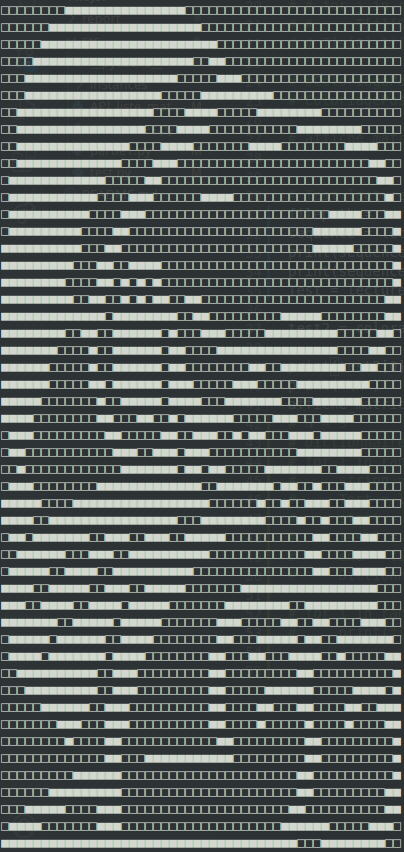
\includegraphics[scale=0.4]{instance9.png}
			\end{center}
		
			\paragraph{Q11}
				L'algorithme implémenté dans cette partie ne sait pas résoudre l'instance 11.txt car pour chaque ligne et pour chaque colonnes, les fonctions \textit{ColoreLig} et \textit{ColoreCol} ne permettent pas de colorier des cases.
	
	
	\section{Méthode de résolution complète}
		
		\paragraph{Q12}
		
			La fonction \textit{EnumRec} est de complexité $ \boxed{O(2^{MN}(N^2 \times M^5 + M^2 \times N^5)) } $. En effet, pour chaque case, on fait deux appels récursifs, une en coloriant la case en blanc, et l'autre en noir, et on fait appel à la fonction \textit{ColorierEtPropager} qui est de même complexité que \textit{Coloration} dans le pire cas. Il y a $ MN $ cases au total, d'où la complexité que nous venons d'énoncer. \\
			Par conséquent, l'algorithme d'énumération a une complexité exponentielle.
		
		\subsection{Implantation et tests}
		
			\paragraph{Q13}
				Il s'agit des fonctions du fichier \textit{src/partie2.py}
		
			\paragraph{Q14}
				Le tableau suivant donne les temps de résolution de chacune des instances 1 à 16 avec l'algorithme de la partie 2.
				\begin{center}
					\begin{tabular}{|c|c|c|c|c|c|c|c|c|c|c| }
						\hline
						instance & 1 & 2 & 3 & 4 & 5 & 6 & 7 & 8 & 9 & 10 \\ \hline
						temps de résolution (s) & 0.00102 & 0.144 & 0.073 & 0.196 & 0.168 & 0.384 & 0.224 & 0.342 & 3.703 & 3.820 \\ \hline
					\end{tabular}
				\end{center}
			
				\begin{center}
					\begin{tabular}{|c|c|c|c|c|c|c| }
						\hline
						instance & 11 & 12 & 13 & 14 & 15 & 16 \\ \hline
						temps de résolution (s) & 0.00031 & 0.384 & 0.449 & 0.332 & 0.402 & 33.510 \\ \hline
					\end{tabular}
				\end{center}
			
				Le tableau suivant donne les temps de résolution de chacune des instances 11 à 16 avec l'algorithme de la partie 1.
				\begin{center}
					\begin{tabular}{|c|c|c|c|c|c|c| }
						\hline
						instance & 11 & 12 & 13 & 14 & 15 & 16 \\ \hline
						temps de résolution (s) & 0.00023 & 0.389 & 0.507 & 0.318 & 0.225 & 0.844 \\ \hline
					\end{tabular}
				\end{center}
				
				On remarque que l'algorithme de coloration et celui d'énumération résolvent complètement les instances 1 à 10 avec un temps de même ordre de grandeur. Pour les instances 11 à 15, rapidement l'algorithme de coloration ne parvient pas à résoudre la grille de jeu tandis que l'algorithme d'énumération, avec un temps de résolution de même ordre de grandeur, y parvient. Pour l'instance 16, ce dernier prend beaucoup de temps, et c'est là que l'on voit la complexité exponentielle de l'algorithme. \\
				
				La grille obtenue pour l'instance 15.txt avec l'algorithme de la partie 1 est la suivante :
				\begin{center}
					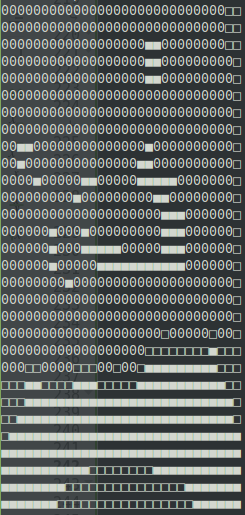
\includegraphics[scale=0.4]{instance15-1.png}
				\end{center}
			
				La grille obtenue pour l'instance 15.txt avec l'algorithme de la partie 2 est la suivante :
				\begin{center}
					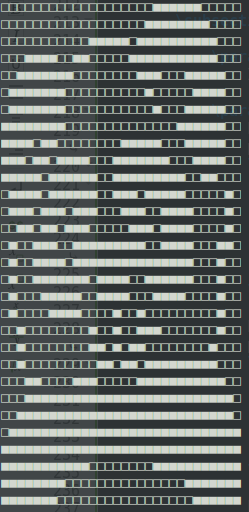
\includegraphics[scale=0.4]{instance15-2.png}
				\end{center}
		
		
		
		
		
		
		
		
		
		
		
		
		
		
		
		
		
		
		
		
		
		
		
		
		
		
		
\end{document}